\documentclass[10pt]{article}
\usepackage[margin=1cm, bottom=2cm]{geometry}
\usepackage{tikz}
\usepackage[urlcolor=blue, colorlinks=true]{hyperref}
\usepackage{longtable}
\usepackage{multirow}

\begin{document}

\title{Report\\Assignment 1: The Matrix Universe}
\author{Timur Usmanov, B23-ISE-01}
\date{October 29, 2024}
\maketitle

\section*{Introduction}
Find the complete source code and tests at \url{https://github.com/Error10556/IntroToAI1}.

\section{PEAS Description}

In this problem, the Actor has to find the smallest number of moves required to reach the destination cell.

\begin{enumerate}
	\item The Actor's performance measures, in order of priority, are:
	\begin{enumerate}
		\item The Actor survives;
		\item The Actor gives the correct answer;
		\item The Actor spends as few moves as possible until he can give an answer.
	\end{enumerate}
	
	\item The Actor's environment is a grid of $9\times 9$ cells, where each cell might contain an Agent, a Sentinel, the Backdoor key, or the Keymaker. This environment is:
	
	\begin{enumerate}
		\item \textbf{Partially observable}, because Neo only sees in a Moore neighborhood of range 1 or 2;
		\item \textbf{Multi-agent}, because, arguably, Agents and Sentinels have to observe their environment and kill Neo, which is an action;
		\item \textbf{Deterministic}, because there are no random elements; the environment is entirely predictable;
		\item \textbf{Sequential}, because the action of picking up the key changes the environment and would require Neo to make different moves;
		\item \textbf{Static}, because the environment does not change while the Actor thinks;
		\item \textbf{Discrete}, because there is only a finite number of states of the environment;
		\item \textbf{Known}, because the rules are given in the assignment.
	\end{enumerate}
	
	\item Neo's actuators are his legs (to make moves) and hands (to pick up the Backdoor key). Formally, the actuator is the \texttt{m x y} command.
	
	\item Neo's sensors are his eyes and the Trinity, which allow him to see the objects on the map and the perceived cells. Formally, our sensor is the standard input stream.
\end{enumerate}

\section{Algorithm flow}
\subsection{A*}
In this algorithm, each known cell is associated with several values: (a) the true shortest distance $d$ from $(0, 0)$ to that cell over safe cells, (b) the Manhattan distance $m$ from that cell to the Keymaker, (c) whether the cell is \textit{safe}, \textit{dangerous}, or \textit{unknown}, (d) whether or not the cell has been visited.
We define the estimate $E(c)$ of cell $c$ as $d + m$.

Neo first observes the surroundings at cell $(0, 0)$. Then, in a cycle, the Actor does the following:\newline
Neo chooses a safe cell $c$ that is adjacent to a previously visited cell, among those~--- with the least $E(c)$, among those~--- with the least $m$, among those~--- the one closest to Neo if he has to walk on safe cells to reach it (the distance is, again, calculated via another A* algorithm). Then, Neo moves there, scanning the surroundings and updating the map. Upon reaching the cell $c$, Neo updates the values associated with the adjacent unvisited cells of $c$. Once we have set the true shortest distance $d$ of the Keymaker cell, we may break out of the cycle. If there are no unvisited cells adjacent to a visited one, we know that there is no answer.

We ignore the Backdoor key, as it ``is not an obligation" ``to utilize its advantages".

\subsection{Backtracking}
In this algorithm, each known cell might be: (a) visited or unvisited, (b) safe or unsafe.

Neo explores the safe and reachable portion of the map using Depth-First Search (DFS). DFS marks cells as visited upon reaching them and does not explore already visited cells. When there are no adjacent unvisited cells, Neo backtracks.
After the execution of DFS, we use a Breadth-First Search on the explored part of the map to find the shortest distance to the Keymaker. If the Keymaker is not in the reachable portion, we output \texttt{-1}.

Again, we ignore the Backdoor key.

\section{Statistical analysis}
\subsection{Impossible tests}
A total of $1000$ tests were generated, out of which exactly 10 have no path to the Keymaker (if we ignore the Backdoor key).

\begin{center}

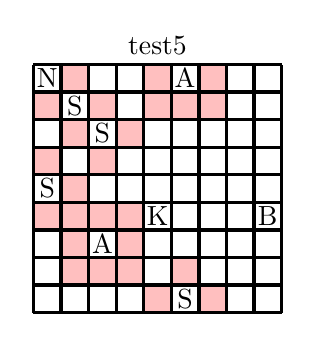
\begin{tikzpicture}[scale=0.35,baseline=0]\node[above] at (4.5,0) {test5};
	\node at (0.5,-0.5) {N};
	\fill[pink] (0,-1) rectangle (1,-2);
	\fill[pink] (0,-3) rectangle (1,-4);
	\node at (0.5,-4.5) {S};
	\fill[pink] (0,-5) rectangle (1,-6);
	\fill[pink] (1,0) rectangle (2,-1);
	\node at (1.5,-1.5) {S};
	\fill[pink] (1,-2) rectangle (2,-3);
	\fill[pink] (1,-4) rectangle (2,-5);
	\fill[pink] (1,-5) rectangle (2,-6);
	\fill[pink] (1,-6) rectangle (2,-7);
	\fill[pink] (1,-7) rectangle (2,-8);
	\fill[pink] (2,-1) rectangle (3,-2);
	\node at (2.5,-2.5) {S};
	\fill[pink] (2,-3) rectangle (3,-4);
	\fill[pink] (2,-5) rectangle (3,-6);
	\node at (2.5,-6.5) {A};
	\fill[pink] (2,-7) rectangle (3,-8);
	\fill[pink] (3,-2) rectangle (4,-3);
	\fill[pink] (3,-5) rectangle (4,-6);
	\fill[pink] (3,-6) rectangle (4,-7);
	\fill[pink] (3,-7) rectangle (4,-8);
	\fill[pink] (4,0) rectangle (5,-1);
	\fill[pink] (4,-1) rectangle (5,-2);
	\node at (4.5,-5.5) {K};
	\fill[pink] (4,-8) rectangle (5,-9);
	\node at (5.5,-0.5) {A};
	\fill[pink] (5,-1) rectangle (6,-2);
	\fill[pink] (5,-7) rectangle (6,-8);
	\node at (5.5,-8.5) {S};
	\fill[pink] (6,0) rectangle (7,-1);
	\fill[pink] (6,-1) rectangle (7,-2);
	\fill[pink] (6,-8) rectangle (7,-9);
	\node at (8.5,-5.5) {B};
	\draw[very thick, step=1.0] (0,0) grid (9,-9);
\end{tikzpicture}
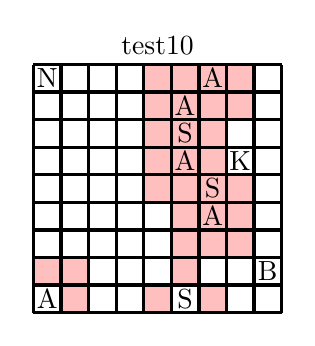
\begin{tikzpicture}[scale=0.35,baseline=0]\node[above] at (4.5,0) {test10};
	\node at (0.5,-0.5) {N};
	\fill[pink] (0,-7) rectangle (1,-8);
	\node at (0.5,-8.5) {A};
	\fill[pink] (1,-7) rectangle (2,-8);
	\fill[pink] (1,-8) rectangle (2,-9);
	\fill[pink] (4,0) rectangle (5,-1);
	\fill[pink] (4,-1) rectangle (5,-2);
	\fill[pink] (4,-2) rectangle (5,-3);
	\fill[pink] (4,-3) rectangle (5,-4);
	\fill[pink] (4,-4) rectangle (5,-5);
	\fill[pink] (4,-8) rectangle (5,-9);
	\fill[pink] (5,0) rectangle (6,-1);
	\fill[pink] (5,-1) rectangle (6,-2);
	\node at (5.5,-1.5) {A};
	\fill[pink] (5,-2) rectangle (6,-3);
	\node at (5.5,-2.5) {S};
	\fill[pink] (5,-3) rectangle (6,-4);
	\node at (5.5,-3.5) {A};
	\fill[pink] (5,-4) rectangle (6,-5);
	\fill[pink] (5,-5) rectangle (6,-6);
	\fill[pink] (5,-6) rectangle (6,-7);
	\fill[pink] (5,-7) rectangle (6,-8);
	\node at (5.5,-8.5) {S};
	\fill[pink] (6,0) rectangle (7,-1);
	\node at (6.5,-0.5) {A};
	\fill[pink] (6,-1) rectangle (7,-2);
	\fill[pink] (6,-2) rectangle (7,-3);
	\fill[pink] (6,-3) rectangle (7,-4);
	\fill[pink] (6,-4) rectangle (7,-5);
	\node at (6.5,-4.5) {S};
	\fill[pink] (6,-5) rectangle (7,-6);
	\node at (6.5,-5.5) {A};
	\fill[pink] (6,-6) rectangle (7,-7);
	\fill[pink] (6,-8) rectangle (7,-9);
	\fill[pink] (7,0) rectangle (8,-1);
	\fill[pink] (7,-1) rectangle (8,-2);
	\node at (7.5,-3.5) {K};
	\fill[pink] (7,-4) rectangle (8,-5);
	\fill[pink] (7,-5) rectangle (8,-6);
	\fill[pink] (7,-6) rectangle (8,-7);
	\node at (8.5,-7.5) {B};
	\draw[very thick, step=1.0] (0,0) grid (9,-9);
\end{tikzpicture}
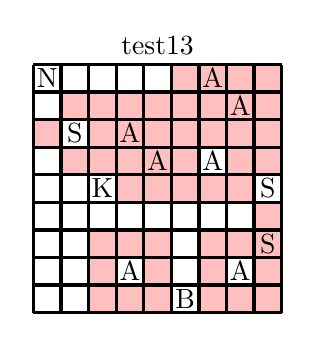
\begin{tikzpicture}[scale=0.35,baseline=0]\node[above] at (4.5,0) {test13};
	\node at (0.5,-0.5) {N};
	\fill[pink] (0,-2) rectangle (1,-3);
	\fill[pink] (1,-1) rectangle (2,-2);
	\node at (1.5,-2.5) {S};
	\fill[pink] (1,-3) rectangle (2,-4);
	\fill[pink] (2,-1) rectangle (3,-2);
	\fill[pink] (2,-2) rectangle (3,-3);
	\fill[pink] (2,-3) rectangle (3,-4);
	\node at (2.5,-4.5) {K};
	\fill[pink] (2,-6) rectangle (3,-7);
	\fill[pink] (2,-7) rectangle (3,-8);
	\fill[pink] (2,-8) rectangle (3,-9);
	\fill[pink] (3,-1) rectangle (4,-2);
	\fill[pink] (3,-2) rectangle (4,-3);
	\node at (3.5,-2.5) {A};
	\fill[pink] (3,-3) rectangle (4,-4);
	\fill[pink] (3,-4) rectangle (4,-5);
	\fill[pink] (3,-6) rectangle (4,-7);
	\node at (3.5,-7.5) {A};
	\fill[pink] (3,-8) rectangle (4,-9);
	\fill[pink] (4,-1) rectangle (5,-2);
	\fill[pink] (4,-2) rectangle (5,-3);
	\fill[pink] (4,-3) rectangle (5,-4);
	\node at (4.5,-3.5) {A};
	\fill[pink] (4,-4) rectangle (5,-5);
	\fill[pink] (4,-6) rectangle (5,-7);
	\fill[pink] (4,-7) rectangle (5,-8);
	\fill[pink] (4,-8) rectangle (5,-9);
	\fill[pink] (5,0) rectangle (6,-1);
	\fill[pink] (5,-1) rectangle (6,-2);
	\fill[pink] (5,-2) rectangle (6,-3);
	\fill[pink] (5,-3) rectangle (6,-4);
	\fill[pink] (5,-4) rectangle (6,-5);
	\node at (5.5,-8.5) {B};
	\fill[pink] (6,0) rectangle (7,-1);
	\node at (6.5,-0.5) {A};
	\fill[pink] (6,-1) rectangle (7,-2);
	\fill[pink] (6,-2) rectangle (7,-3);
	\node at (6.5,-3.5) {A};
	\fill[pink] (6,-4) rectangle (7,-5);
	\fill[pink] (6,-6) rectangle (7,-7);
	\fill[pink] (6,-7) rectangle (7,-8);
	\fill[pink] (6,-8) rectangle (7,-9);
	\fill[pink] (7,0) rectangle (8,-1);
	\fill[pink] (7,-1) rectangle (8,-2);
	\node at (7.5,-1.5) {A};
	\fill[pink] (7,-2) rectangle (8,-3);
	\fill[pink] (7,-3) rectangle (8,-4);
	\fill[pink] (7,-4) rectangle (8,-5);
	\fill[pink] (7,-6) rectangle (8,-7);
	\node at (7.5,-7.5) {A};
	\fill[pink] (7,-8) rectangle (8,-9);
	\fill[pink] (8,0) rectangle (9,-1);
	\fill[pink] (8,-1) rectangle (9,-2);
	\fill[pink] (8,-2) rectangle (9,-3);
	\fill[pink] (8,-3) rectangle (9,-4);
	\node at (8.5,-4.5) {S};
	\fill[pink] (8,-5) rectangle (9,-6);
	\fill[pink] (8,-6) rectangle (9,-7);
	\node at (8.5,-6.5) {S};
	\fill[pink] (8,-7) rectangle (9,-8);
	\fill[pink] (8,-8) rectangle (9,-9);
	\draw[very thick, step=1.0] (0,0) grid (9,-9);
\end{tikzpicture}
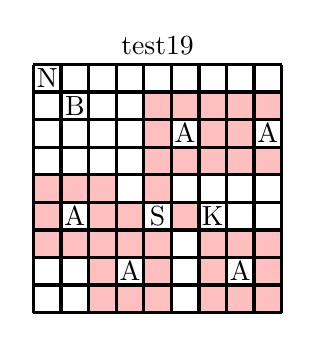
\begin{tikzpicture}[scale=0.35,baseline=0]\node[above] at (4.5,0) {test19};
	\node at (0.5,-0.5) {N};
	\fill[pink] (0,-4) rectangle (1,-5);
	\fill[pink] (0,-5) rectangle (1,-6);
	\fill[pink] (0,-6) rectangle (1,-7);
	\node at (1.5,-1.5) {B};
	\fill[pink] (1,-4) rectangle (2,-5);
	\node at (1.5,-5.5) {A};
	\fill[pink] (1,-6) rectangle (2,-7);
	\fill[pink] (2,-4) rectangle (3,-5);
	\fill[pink] (2,-5) rectangle (3,-6);
	\fill[pink] (2,-6) rectangle (3,-7);
	\fill[pink] (2,-7) rectangle (3,-8);
	\fill[pink] (2,-8) rectangle (3,-9);
	\fill[pink] (3,-5) rectangle (4,-6);
	\fill[pink] (3,-6) rectangle (4,-7);
	\node at (3.5,-7.5) {A};
	\fill[pink] (3,-8) rectangle (4,-9);
	\fill[pink] (4,-1) rectangle (5,-2);
	\fill[pink] (4,-2) rectangle (5,-3);
	\fill[pink] (4,-3) rectangle (5,-4);
	\fill[pink] (4,-4) rectangle (5,-5);
	\node at (4.5,-5.5) {S};
	\fill[pink] (4,-6) rectangle (5,-7);
	\fill[pink] (4,-7) rectangle (5,-8);
	\fill[pink] (4,-8) rectangle (5,-9);
	\fill[pink] (5,-1) rectangle (6,-2);
	\node at (5.5,-2.5) {A};
	\fill[pink] (5,-3) rectangle (6,-4);
	\fill[pink] (5,-5) rectangle (6,-6);
	\fill[pink] (6,-1) rectangle (7,-2);
	\fill[pink] (6,-2) rectangle (7,-3);
	\fill[pink] (6,-3) rectangle (7,-4);
	\node at (6.5,-5.5) {K};
	\fill[pink] (6,-6) rectangle (7,-7);
	\fill[pink] (6,-7) rectangle (7,-8);
	\fill[pink] (6,-8) rectangle (7,-9);
	\fill[pink] (7,-1) rectangle (8,-2);
	\fill[pink] (7,-2) rectangle (8,-3);
	\fill[pink] (7,-3) rectangle (8,-4);
	\fill[pink] (7,-6) rectangle (8,-7);
	\node at (7.5,-7.5) {A};
	\fill[pink] (7,-8) rectangle (8,-9);
	\fill[pink] (8,-1) rectangle (9,-2);
	\node at (8.5,-2.5) {A};
	\fill[pink] (8,-3) rectangle (9,-4);
	\fill[pink] (8,-6) rectangle (9,-7);
	\fill[pink] (8,-7) rectangle (9,-8);
	\fill[pink] (8,-8) rectangle (9,-9);
	\draw[very thick, step=1.0] (0,0) grid (9,-9);
\end{tikzpicture}
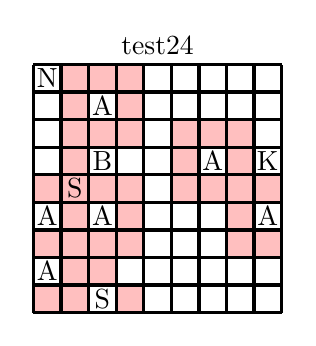
\begin{tikzpicture}[scale=0.35,baseline=0]\node[above] at (4.5,0) {test24};
	\node at (0.5,-0.5) {N};
	\fill[pink] (0,-4) rectangle (1,-5);
	\node at (0.5,-5.5) {A};
	\fill[pink] (0,-6) rectangle (1,-7);
	\node at (0.5,-7.5) {A};
	\fill[pink] (0,-8) rectangle (1,-9);
	\fill[pink] (1,0) rectangle (2,-1);
	\fill[pink] (1,-1) rectangle (2,-2);
	\fill[pink] (1,-2) rectangle (2,-3);
	\fill[pink] (1,-3) rectangle (2,-4);
	\fill[pink] (1,-4) rectangle (2,-5);
	\node at (1.5,-4.5) {S};
	\fill[pink] (1,-5) rectangle (2,-6);
	\fill[pink] (1,-6) rectangle (2,-7);
	\fill[pink] (1,-7) rectangle (2,-8);
	\fill[pink] (1,-8) rectangle (2,-9);
	\fill[pink] (2,0) rectangle (3,-1);
	\node at (2.5,-1.5) {A};
	\fill[pink] (2,-2) rectangle (3,-3);
	\node at (2.5,-3.5) {B};
	\fill[pink] (2,-4) rectangle (3,-5);
	\node at (2.5,-5.5) {A};
	\fill[pink] (2,-6) rectangle (3,-7);
	\fill[pink] (2,-7) rectangle (3,-8);
	\node at (2.5,-8.5) {S};
	\fill[pink] (3,0) rectangle (4,-1);
	\fill[pink] (3,-1) rectangle (4,-2);
	\fill[pink] (3,-2) rectangle (4,-3);
	\fill[pink] (3,-4) rectangle (4,-5);
	\fill[pink] (3,-5) rectangle (4,-6);
	\fill[pink] (3,-6) rectangle (4,-7);
	\fill[pink] (3,-8) rectangle (4,-9);
	\fill[pink] (5,-2) rectangle (6,-3);
	\fill[pink] (5,-3) rectangle (6,-4);
	\fill[pink] (5,-4) rectangle (6,-5);
	\fill[pink] (6,-2) rectangle (7,-3);
	\node at (6.5,-3.5) {A};
	\fill[pink] (6,-4) rectangle (7,-5);
	\fill[pink] (7,-2) rectangle (8,-3);
	\fill[pink] (7,-3) rectangle (8,-4);
	\fill[pink] (7,-4) rectangle (8,-5);
	\fill[pink] (7,-5) rectangle (8,-6);
	\fill[pink] (7,-6) rectangle (8,-7);
	\node at (8.5,-3.5) {K};
	\fill[pink] (8,-4) rectangle (9,-5);
	\node at (8.5,-5.5) {A};
	\fill[pink] (8,-6) rectangle (9,-7);
	\draw[very thick, step=1.0] (0,0) grid (9,-9);
\end{tikzpicture}
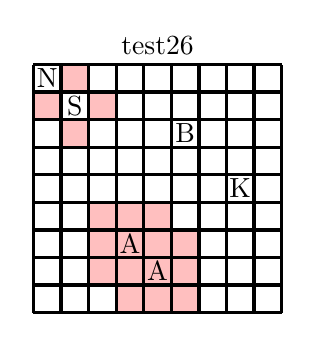
\begin{tikzpicture}[scale=0.35,baseline=0]\node[above] at (4.5,0) {test26};
	\node at (0.5,-0.5) {N};
	\fill[pink] (0,-1) rectangle (1,-2);
	\fill[pink] (1,0) rectangle (2,-1);
	\node at (1.5,-1.5) {S};
	\fill[pink] (1,-2) rectangle (2,-3);
	\fill[pink] (2,-1) rectangle (3,-2);
	\fill[pink] (2,-5) rectangle (3,-6);
	\fill[pink] (2,-6) rectangle (3,-7);
	\fill[pink] (2,-7) rectangle (3,-8);
	\fill[pink] (3,-5) rectangle (4,-6);
	\fill[pink] (3,-6) rectangle (4,-7);
	\node at (3.5,-6.5) {A};
	\fill[pink] (3,-7) rectangle (4,-8);
	\fill[pink] (3,-8) rectangle (4,-9);
	\fill[pink] (4,-5) rectangle (5,-6);
	\fill[pink] (4,-6) rectangle (5,-7);
	\fill[pink] (4,-7) rectangle (5,-8);
	\node at (4.5,-7.5) {A};
	\fill[pink] (4,-8) rectangle (5,-9);
	\node at (5.5,-2.5) {B};
	\fill[pink] (5,-6) rectangle (6,-7);
	\fill[pink] (5,-7) rectangle (6,-8);
	\fill[pink] (5,-8) rectangle (6,-9);
	\node at (7.5,-4.5) {K};
	\draw[very thick, step=1.0] (0,0) grid (9,-9);
\end{tikzpicture}
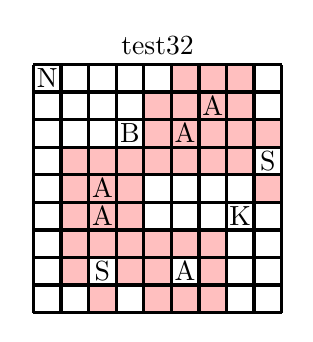
\begin{tikzpicture}[scale=0.35,baseline=0]\node[above] at (4.5,0) {test32};
	\node at (0.5,-0.5) {N};
	\fill[pink] (1,-3) rectangle (2,-4);
	\fill[pink] (1,-4) rectangle (2,-5);
	\fill[pink] (1,-5) rectangle (2,-6);
	\fill[pink] (1,-6) rectangle (2,-7);
	\fill[pink] (1,-7) rectangle (2,-8);
	\fill[pink] (2,-3) rectangle (3,-4);
	\fill[pink] (2,-4) rectangle (3,-5);
	\node at (2.5,-4.5) {A};
	\fill[pink] (2,-5) rectangle (3,-6);
	\node at (2.5,-5.5) {A};
	\fill[pink] (2,-6) rectangle (3,-7);
	\node at (2.5,-7.5) {S};
	\fill[pink] (2,-8) rectangle (3,-9);
	\node at (3.5,-2.5) {B};
	\fill[pink] (3,-3) rectangle (4,-4);
	\fill[pink] (3,-4) rectangle (4,-5);
	\fill[pink] (3,-5) rectangle (4,-6);
	\fill[pink] (3,-6) rectangle (4,-7);
	\fill[pink] (3,-7) rectangle (4,-8);
	\fill[pink] (4,-1) rectangle (5,-2);
	\fill[pink] (4,-2) rectangle (5,-3);
	\fill[pink] (4,-3) rectangle (5,-4);
	\fill[pink] (4,-6) rectangle (5,-7);
	\fill[pink] (4,-7) rectangle (5,-8);
	\fill[pink] (4,-8) rectangle (5,-9);
	\fill[pink] (5,0) rectangle (6,-1);
	\fill[pink] (5,-1) rectangle (6,-2);
	\fill[pink] (5,-2) rectangle (6,-3);
	\node at (5.5,-2.5) {A};
	\fill[pink] (5,-3) rectangle (6,-4);
	\fill[pink] (5,-6) rectangle (6,-7);
	\node at (5.5,-7.5) {A};
	\fill[pink] (5,-8) rectangle (6,-9);
	\fill[pink] (6,0) rectangle (7,-1);
	\fill[pink] (6,-1) rectangle (7,-2);
	\node at (6.5,-1.5) {A};
	\fill[pink] (6,-2) rectangle (7,-3);
	\fill[pink] (6,-3) rectangle (7,-4);
	\fill[pink] (6,-6) rectangle (7,-7);
	\fill[pink] (6,-7) rectangle (7,-8);
	\fill[pink] (6,-8) rectangle (7,-9);
	\fill[pink] (7,0) rectangle (8,-1);
	\fill[pink] (7,-1) rectangle (8,-2);
	\fill[pink] (7,-2) rectangle (8,-3);
	\fill[pink] (7,-3) rectangle (8,-4);
	\node at (7.5,-5.5) {K};
	\fill[pink] (8,-2) rectangle (9,-3);
	\node at (8.5,-3.5) {S};
	\fill[pink] (8,-4) rectangle (9,-5);
	\draw[very thick, step=1.0] (0,0) grid (9,-9);
\end{tikzpicture}
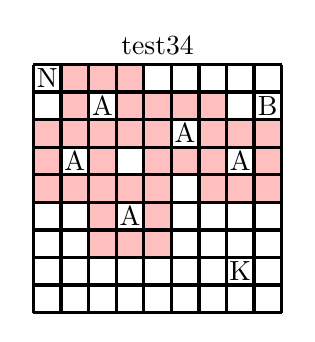
\begin{tikzpicture}[scale=0.35,baseline=0]\node[above] at (4.5,0) {test34};
	\node at (0.5,-0.5) {N};
	\fill[pink] (0,-2) rectangle (1,-3);
	\fill[pink] (0,-3) rectangle (1,-4);
	\fill[pink] (0,-4) rectangle (1,-5);
	\fill[pink] (1,0) rectangle (2,-1);
	\fill[pink] (1,-1) rectangle (2,-2);
	\fill[pink] (1,-2) rectangle (2,-3);
	\node at (1.5,-3.5) {A};
	\fill[pink] (1,-4) rectangle (2,-5);
	\fill[pink] (2,0) rectangle (3,-1);
	\node at (2.5,-1.5) {A};
	\fill[pink] (2,-2) rectangle (3,-3);
	\fill[pink] (2,-3) rectangle (3,-4);
	\fill[pink] (2,-4) rectangle (3,-5);
	\fill[pink] (2,-5) rectangle (3,-6);
	\fill[pink] (2,-6) rectangle (3,-7);
	\fill[pink] (3,0) rectangle (4,-1);
	\fill[pink] (3,-1) rectangle (4,-2);
	\fill[pink] (3,-2) rectangle (4,-3);
	\fill[pink] (3,-4) rectangle (4,-5);
	\node at (3.5,-5.5) {A};
	\fill[pink] (3,-6) rectangle (4,-7);
	\fill[pink] (4,-1) rectangle (5,-2);
	\fill[pink] (4,-2) rectangle (5,-3);
	\fill[pink] (4,-3) rectangle (5,-4);
	\fill[pink] (4,-4) rectangle (5,-5);
	\fill[pink] (4,-5) rectangle (5,-6);
	\fill[pink] (4,-6) rectangle (5,-7);
	\fill[pink] (5,-1) rectangle (6,-2);
	\node at (5.5,-2.5) {A};
	\fill[pink] (5,-3) rectangle (6,-4);
	\fill[pink] (6,-1) rectangle (7,-2);
	\fill[pink] (6,-2) rectangle (7,-3);
	\fill[pink] (6,-3) rectangle (7,-4);
	\fill[pink] (6,-4) rectangle (7,-5);
	\fill[pink] (7,-2) rectangle (8,-3);
	\node at (7.5,-3.5) {A};
	\fill[pink] (7,-4) rectangle (8,-5);
	\node at (7.5,-7.5) {K};
	\node at (8.5,-1.5) {B};
	\fill[pink] (8,-2) rectangle (9,-3);
	\fill[pink] (8,-3) rectangle (9,-4);
	\fill[pink] (8,-4) rectangle (9,-5);
	\draw[very thick, step=1.0] (0,0) grid (9,-9);
\end{tikzpicture}
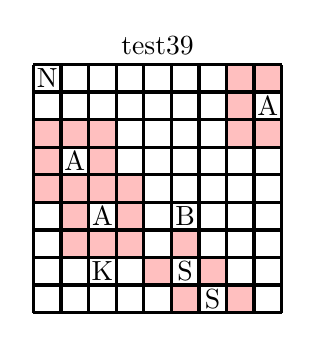
\begin{tikzpicture}[scale=0.35,baseline=0]\node[above] at (4.5,0) {test39};
	\node at (0.5,-0.5) {N};
	\fill[pink] (0,-2) rectangle (1,-3);
	\fill[pink] (0,-3) rectangle (1,-4);
	\fill[pink] (0,-4) rectangle (1,-5);
	\fill[pink] (1,-2) rectangle (2,-3);
	\node at (1.5,-3.5) {A};
	\fill[pink] (1,-4) rectangle (2,-5);
	\fill[pink] (1,-5) rectangle (2,-6);
	\fill[pink] (1,-6) rectangle (2,-7);
	\fill[pink] (2,-2) rectangle (3,-3);
	\fill[pink] (2,-3) rectangle (3,-4);
	\fill[pink] (2,-4) rectangle (3,-5);
	\node at (2.5,-5.5) {A};
	\fill[pink] (2,-6) rectangle (3,-7);
	\node at (2.5,-7.5) {K};
	\fill[pink] (3,-4) rectangle (4,-5);
	\fill[pink] (3,-5) rectangle (4,-6);
	\fill[pink] (3,-6) rectangle (4,-7);
	\fill[pink] (4,-7) rectangle (5,-8);
	\node at (5.5,-5.5) {B};
	\fill[pink] (5,-6) rectangle (6,-7);
	\node at (5.5,-7.5) {S};
	\fill[pink] (5,-8) rectangle (6,-9);
	\fill[pink] (6,-7) rectangle (7,-8);
	\node at (6.5,-8.5) {S};
	\fill[pink] (7,0) rectangle (8,-1);
	\fill[pink] (7,-1) rectangle (8,-2);
	\fill[pink] (7,-2) rectangle (8,-3);
	\fill[pink] (7,-8) rectangle (8,-9);
	\fill[pink] (8,0) rectangle (9,-1);
	\node at (8.5,-1.5) {A};
	\fill[pink] (8,-2) rectangle (9,-3);
	\draw[very thick, step=1.0] (0,0) grid (9,-9);
\end{tikzpicture}
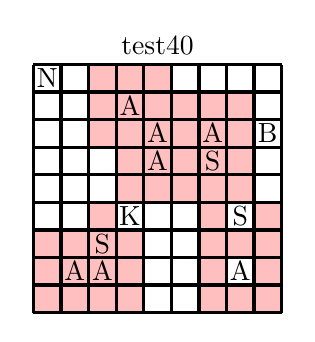
\begin{tikzpicture}[scale=0.35,baseline=0]\node[above] at (4.5,0) {test40};
	\node at (0.5,-0.5) {N};
	\fill[pink] (0,-6) rectangle (1,-7);
	\fill[pink] (0,-7) rectangle (1,-8);
	\fill[pink] (0,-8) rectangle (1,-9);
	\fill[pink] (1,-6) rectangle (2,-7);
	\fill[pink] (1,-7) rectangle (2,-8);
	\node at (1.5,-7.5) {A};
	\fill[pink] (1,-8) rectangle (2,-9);
	\fill[pink] (2,0) rectangle (3,-1);
	\fill[pink] (2,-1) rectangle (3,-2);
	\fill[pink] (2,-2) rectangle (3,-3);
	\fill[pink] (2,-5) rectangle (3,-6);
	\fill[pink] (2,-6) rectangle (3,-7);
	\node at (2.5,-6.5) {S};
	\fill[pink] (2,-7) rectangle (3,-8);
	\node at (2.5,-7.5) {A};
	\fill[pink] (2,-8) rectangle (3,-9);
	\fill[pink] (3,0) rectangle (4,-1);
	\fill[pink] (3,-1) rectangle (4,-2);
	\node at (3.5,-1.5) {A};
	\fill[pink] (3,-2) rectangle (4,-3);
	\fill[pink] (3,-3) rectangle (4,-4);
	\fill[pink] (3,-4) rectangle (4,-5);
	\node at (3.5,-5.5) {K};
	\fill[pink] (3,-6) rectangle (4,-7);
	\fill[pink] (3,-7) rectangle (4,-8);
	\fill[pink] (3,-8) rectangle (4,-9);
	\fill[pink] (4,0) rectangle (5,-1);
	\fill[pink] (4,-1) rectangle (5,-2);
	\fill[pink] (4,-2) rectangle (5,-3);
	\node at (4.5,-2.5) {A};
	\fill[pink] (4,-3) rectangle (5,-4);
	\node at (4.5,-3.5) {A};
	\fill[pink] (4,-4) rectangle (5,-5);
	\fill[pink] (5,-1) rectangle (6,-2);
	\fill[pink] (5,-2) rectangle (6,-3);
	\fill[pink] (5,-3) rectangle (6,-4);
	\fill[pink] (5,-4) rectangle (6,-5);
	\fill[pink] (6,-1) rectangle (7,-2);
	\fill[pink] (6,-2) rectangle (7,-3);
	\node at (6.5,-2.5) {A};
	\fill[pink] (6,-3) rectangle (7,-4);
	\node at (6.5,-3.5) {S};
	\fill[pink] (6,-4) rectangle (7,-5);
	\fill[pink] (6,-5) rectangle (7,-6);
	\fill[pink] (6,-6) rectangle (7,-7);
	\fill[pink] (6,-7) rectangle (7,-8);
	\fill[pink] (6,-8) rectangle (7,-9);
	\fill[pink] (7,-1) rectangle (8,-2);
	\fill[pink] (7,-2) rectangle (8,-3);
	\fill[pink] (7,-3) rectangle (8,-4);
	\fill[pink] (7,-4) rectangle (8,-5);
	\node at (7.5,-5.5) {S};
	\fill[pink] (7,-6) rectangle (8,-7);
	\node at (7.5,-7.5) {A};
	\fill[pink] (7,-8) rectangle (8,-9);
	\node at (8.5,-2.5) {B};
	\fill[pink] (8,-5) rectangle (9,-6);
	\fill[pink] (8,-6) rectangle (9,-7);
	\fill[pink] (8,-7) rectangle (9,-8);
	\fill[pink] (8,-8) rectangle (9,-9);
	\draw[very thick, step=1.0] (0,0) grid (9,-9);
\end{tikzpicture}
\end{center}
\begin{flushright}
\textit{Legend:} \textbf{N}~--- Neo, \textbf{A}~--- Agent, \textbf{S}~--- Sentinel, \textbf{B}~--- Backdoor key, \textbf{K}~--- Keymaker, \tikz[baseline=0.1]{\fill[pink] (0,0) rectangle (0.3,0.3)}~--- a perceived cell.
\end{flushright}
\begin{figure}[!h]
\caption{Maps with the answer \texttt{-1}.}\label{impossibletests}
\end{figure}

\subsection{Algorithm comparison}
The assignment does not give the definition of ``wins" and ``losses". To disambiguate, we shall call a ``loss" the situation where the Actor dies, or tries to make an invalid move, or gives a wrong answer. A ``win" shall be the opposite. We shall list the number of tests where an algorithm could not find a safe path to the Keymaker as a separate characteristic.

\begin{longtable}[c]{|c|c|c|c|}
	\hline
	\multicolumn{2}{|c|}{} & \textbf{A*} & \textbf{Backtracking}\\
	\hline
	\endhead
	\multicolumn{4}{|c|}{...}\\ \endfoot
	\endlastfoot
	\multirow{4}{3cm}{Execution time, $\mu s$} & Mean & 1261.51 & 2593.16\\\cline{2-4}
	& Mode & 1196 (8 times) & 2298 (4 times)\\\cline{2-4}
	& Median & 1209.5 & 2707\\\cline{2-4}
	& SD & 244.36 & 493.59\\\hline
	\multirow{4}{3cm}{Number of moves} & Mean & 11.47 & 92.81\\\cline{2-4}
	& Mode & 6 (87 times) & 117 (44 times)\\\cline{2-4}
	& Median & 8 & 101\\\cline{2-4}
	& SD & 11.46 & 30.01\\\hline
	\multicolumn{2}{|c|}{Number of wins (correct answers)} & 1000 (100\%) & 1000 (100\%)\\\hline
	\multicolumn{2}{|c|}{Number of losses (failed tests)} & 0 (0\%) & 0 (0\%) \\\hline
	\multicolumn{2}{|c|}{Number of tests with a positive answer} & 990 (99\%) & 990 (99\%)\\\hline
	\multicolumn{2}{|c|}{Number of tests with answer \texttt{-1}} & 10 (1\%) & 10 (1\%) \\\hline
	
	
\end{longtable}
\begin{table}[!h]
	\caption{Statistics of algorithms side-by-side.} \label{comparison}
\end{table}

\subsection{Discussion}


\end{document}